\documentclass{article}
\usepackage{fancyhdr}
\usepackage{graphicx}
\usepackage{amsmath}
\usepackage[margin=1in]{geometry}

\pagestyle{fancy}
\graphicspath{ {./img/} }

\begin{document}
	\begin{titlepage}
		\begin{center}
			\vspace{1cm}
			{\LARGE\textbf{ROM-Based Finite State Machine}}

			\vspace{1.5cm}
			\textbf{\large Ghassan Arnouk}\\
			
			\vspace{1cm}
			\large SYSC 3006A\\
			\large Summer 2020\\
			\large Lab 1 Report\\
			\large Group 1\\
			
						
			\vspace{2cm}
			\textbf{Instructor:} Michel Sayde\\
			
			\vspace{0.1cm}
			\textbf{TA:} Khalid Almahrog\\
			
			\vspace{0.1cm}
			\textbf{Submitted:} 2020/05/14\\			
		\end{center}
	\end{titlepage}
	
	\lhead{Ghassan Arnouk (Group 1)}
	\rhead{ROM-Based Finite State Machine}
	\pagebreak
	
	\section{Discussion Questions}

		\subsection{What is the minimum ROM Address Bit Width needed to implement Table 1, and why?}
		
		If the number of address bits is m, then the ideal number of words in the bank would be $2^m$. Therefore, the minimum number of bits needed to store eight states is \textbf{three} ($2^3 = 8$) bits. 
		
		\subsection{What is the minimum ROM Data Bit Width needed to implement Table 1, and why?} 
		
		The minimum ROM Data Bit Width is \textbf{six} since three bits are necessary to store the three bits of the output (O2,O1,O0), and three more bits are necessary to store the Next State. The tables have eight bits to store the data but the two most significant bits are zeros and can be ignored.
		
		\subsection{Fill in the following table; it is the content of your FSM ROM that you are going to implement.}
		\begin{table}[!ht]
			\centering
			\caption{Content of the FSM ROM}
			\begin{tabular}{|c|c|c|}
				\hline
				Address & DATA content (binary) & DATA content (Hex)\\
				\hline\hline
				0 & 0010 0011 & 23\\
				\hline
				1 & 0001 1100 & 1c\\
				\hline
				2 & 0000 0000 & 00\\
				\hline
				3 & 0011 0101 & 35\\
				\hline
				4 & 0000 1010 & 0a\\
				\hline
				5 & 0011 1111 & 3f\\
				\hline
				6 & 0000 0110 & 06\\
				\hline
				7 & 0011 1001 & 39\\
				\hline
			\end{tabular}       	
		\end{table}
		
		\pagebreak
		
		\subsection{Show here a screenshot of your final Logisim circuit for your implementation.}
		\begin{figure}[!h]
			\centering
			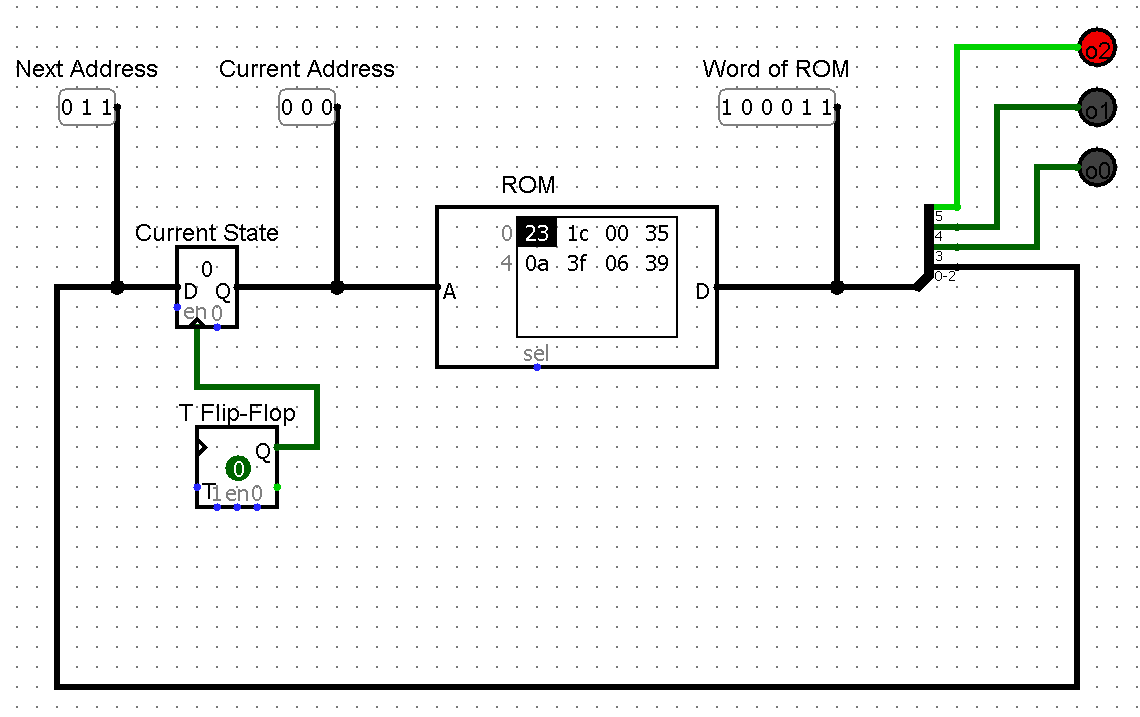
\includegraphics[width=\linewidth]{circuit.png}
			\caption{ROM Circuit Implementation}
		\end{figure}
		
		\subsubsection {A short description of how the component attributes have been configured to meet the lab requirements.}
		
		\begin{itemize}
			\item Toggle Switch: used as a clock input to the Current State Register and is manually toggled to go to the Next State
			\item Register: added as an input to the ROM to hold the Current State and is triggered on the fallingedge of the clock
			\item ROM: contains the content of eight words. The current state is the address of a word in ROM. For example, state 2 corresponds to the word with address 2 in ROM. It is worth mentioning that state 6 forks a child state of its own
			\item Splitter: at the output of the ROM, a splitter is used to split the data into one bundle and three wires:
			\begin{itemize}
				\item a bundle with bits (b2,b1,b0) for the Next state
				\item three separate wires for three outputs (o2,o1,o0)
			\end{itemize}
			\item LEDs: three LEDs are added at the three outputs and the lamps light up when the corresponding output is 1.
		\end{itemize}
		
		\pagebreak
		
		\subsubsection{Insert below a screenshot of your Log table (0.5-mark for the Log table and 1.5-mark for a circuit working properly and respecting the design specifications described in this statement).}
		\begin{table}[!ht]
			\centering
			\caption{Simulation Log Table of the ROM-Based FSM Circuit}			
			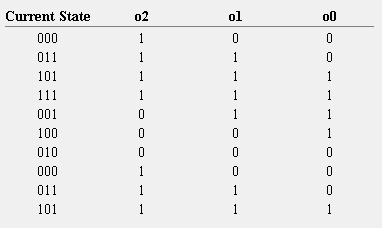
\includegraphics{sim_log_table.png}
		\end{table}				
\end{document}